\chapter{Estimating Diffuse Horizontal Irradiance (DHI) from sky image}
In this chapter, a new approach that we developed for estimating DHI from sky images is explained. First, our experimental setup and data is presented, then we talk about clear-sky model used here, and why estimating DHI is very important in predicting GHI. Furthermore, DHI estimation using the irradiance sensors and also sky-images is discussed. Afterwards, machine learning regression methods for obtaining DHI from sky-image are studies. Finally, the general strategy for power prediction in a photovoltaic power plant using the forecast irradiance components is proposed.

\subsection{Experimental Setup}
This study is conducted on one of the photovoltaic(solar) power plants operated by ABB company. This PV plant which is located in Cavriglia region in Italy is chosen as a pilot site for the "forecasting power prediction using sky-imagery" project. Therefore, it is equipped with the following instruments for recording irradiation and sky images:
\begin{itemize}
\item A customized wide-angle high resolution (4MP) camera system with a fisheye lens covering 185 degrees of field of view. The camera is in a packaging attached to a pole on rooftop of the building next to the site. Figure \ref{fig:camera_on_site} shows the camera and its position next to the PV plates.
\item Two GHI pyranometer (irradiance sensor); located close to the camera on rooftop. One of the sensors is horizontally facing sky, and the other one facing north with around 40 degrees angle to the horizontal plane. It's worth mentioning that the PV plates are titled to south with a fixed angle around 30 degrees to get more sun exposure.  Th sensors are depicted in Figure \ref{fig:pyranometers}.
\item A thermometer for recording the temperature at the site.
\item A PC which is connected to the camera, pyranometers and thermometer via their software interfaces in order to configure sample rates and store taken images and irradiance measurements. The data of power generated by the PV plant is also sampled and stored for every day. All the data recorded during each day is been automatically transfered to the company samba sever at midnight using a control software running on the PC.
\end{itemize}

\begin{figure}[h]
\caption{wide-angle camera system used at Carviglia site}
\label{fig:camera_on_site}
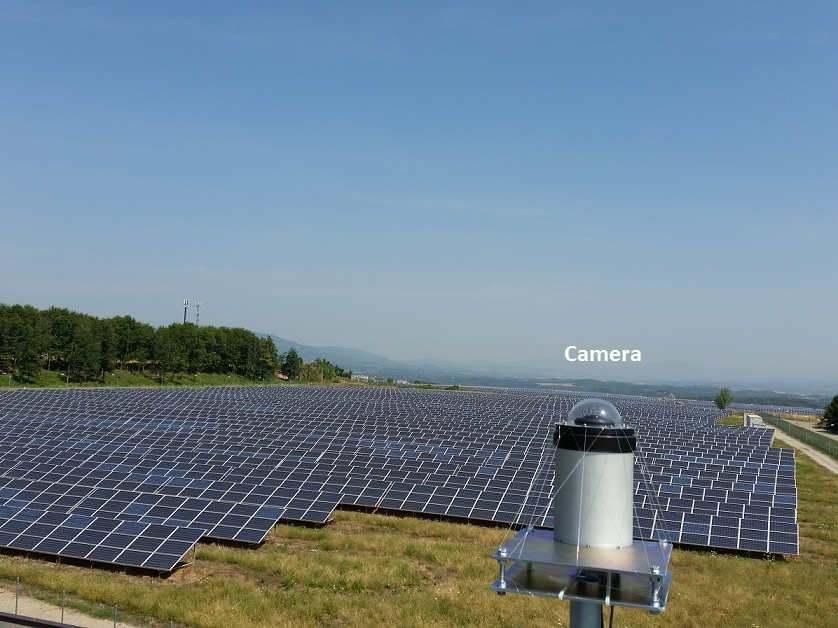
\includegraphics[scale=.3]{camera_on_site}
\centering
\end{figure} 

\begin{figure}[h]
\caption{Two pyranometers (one horizontal, one 45 degrees titled to north) located close to the camera location}
\label{fig:pyranometers}
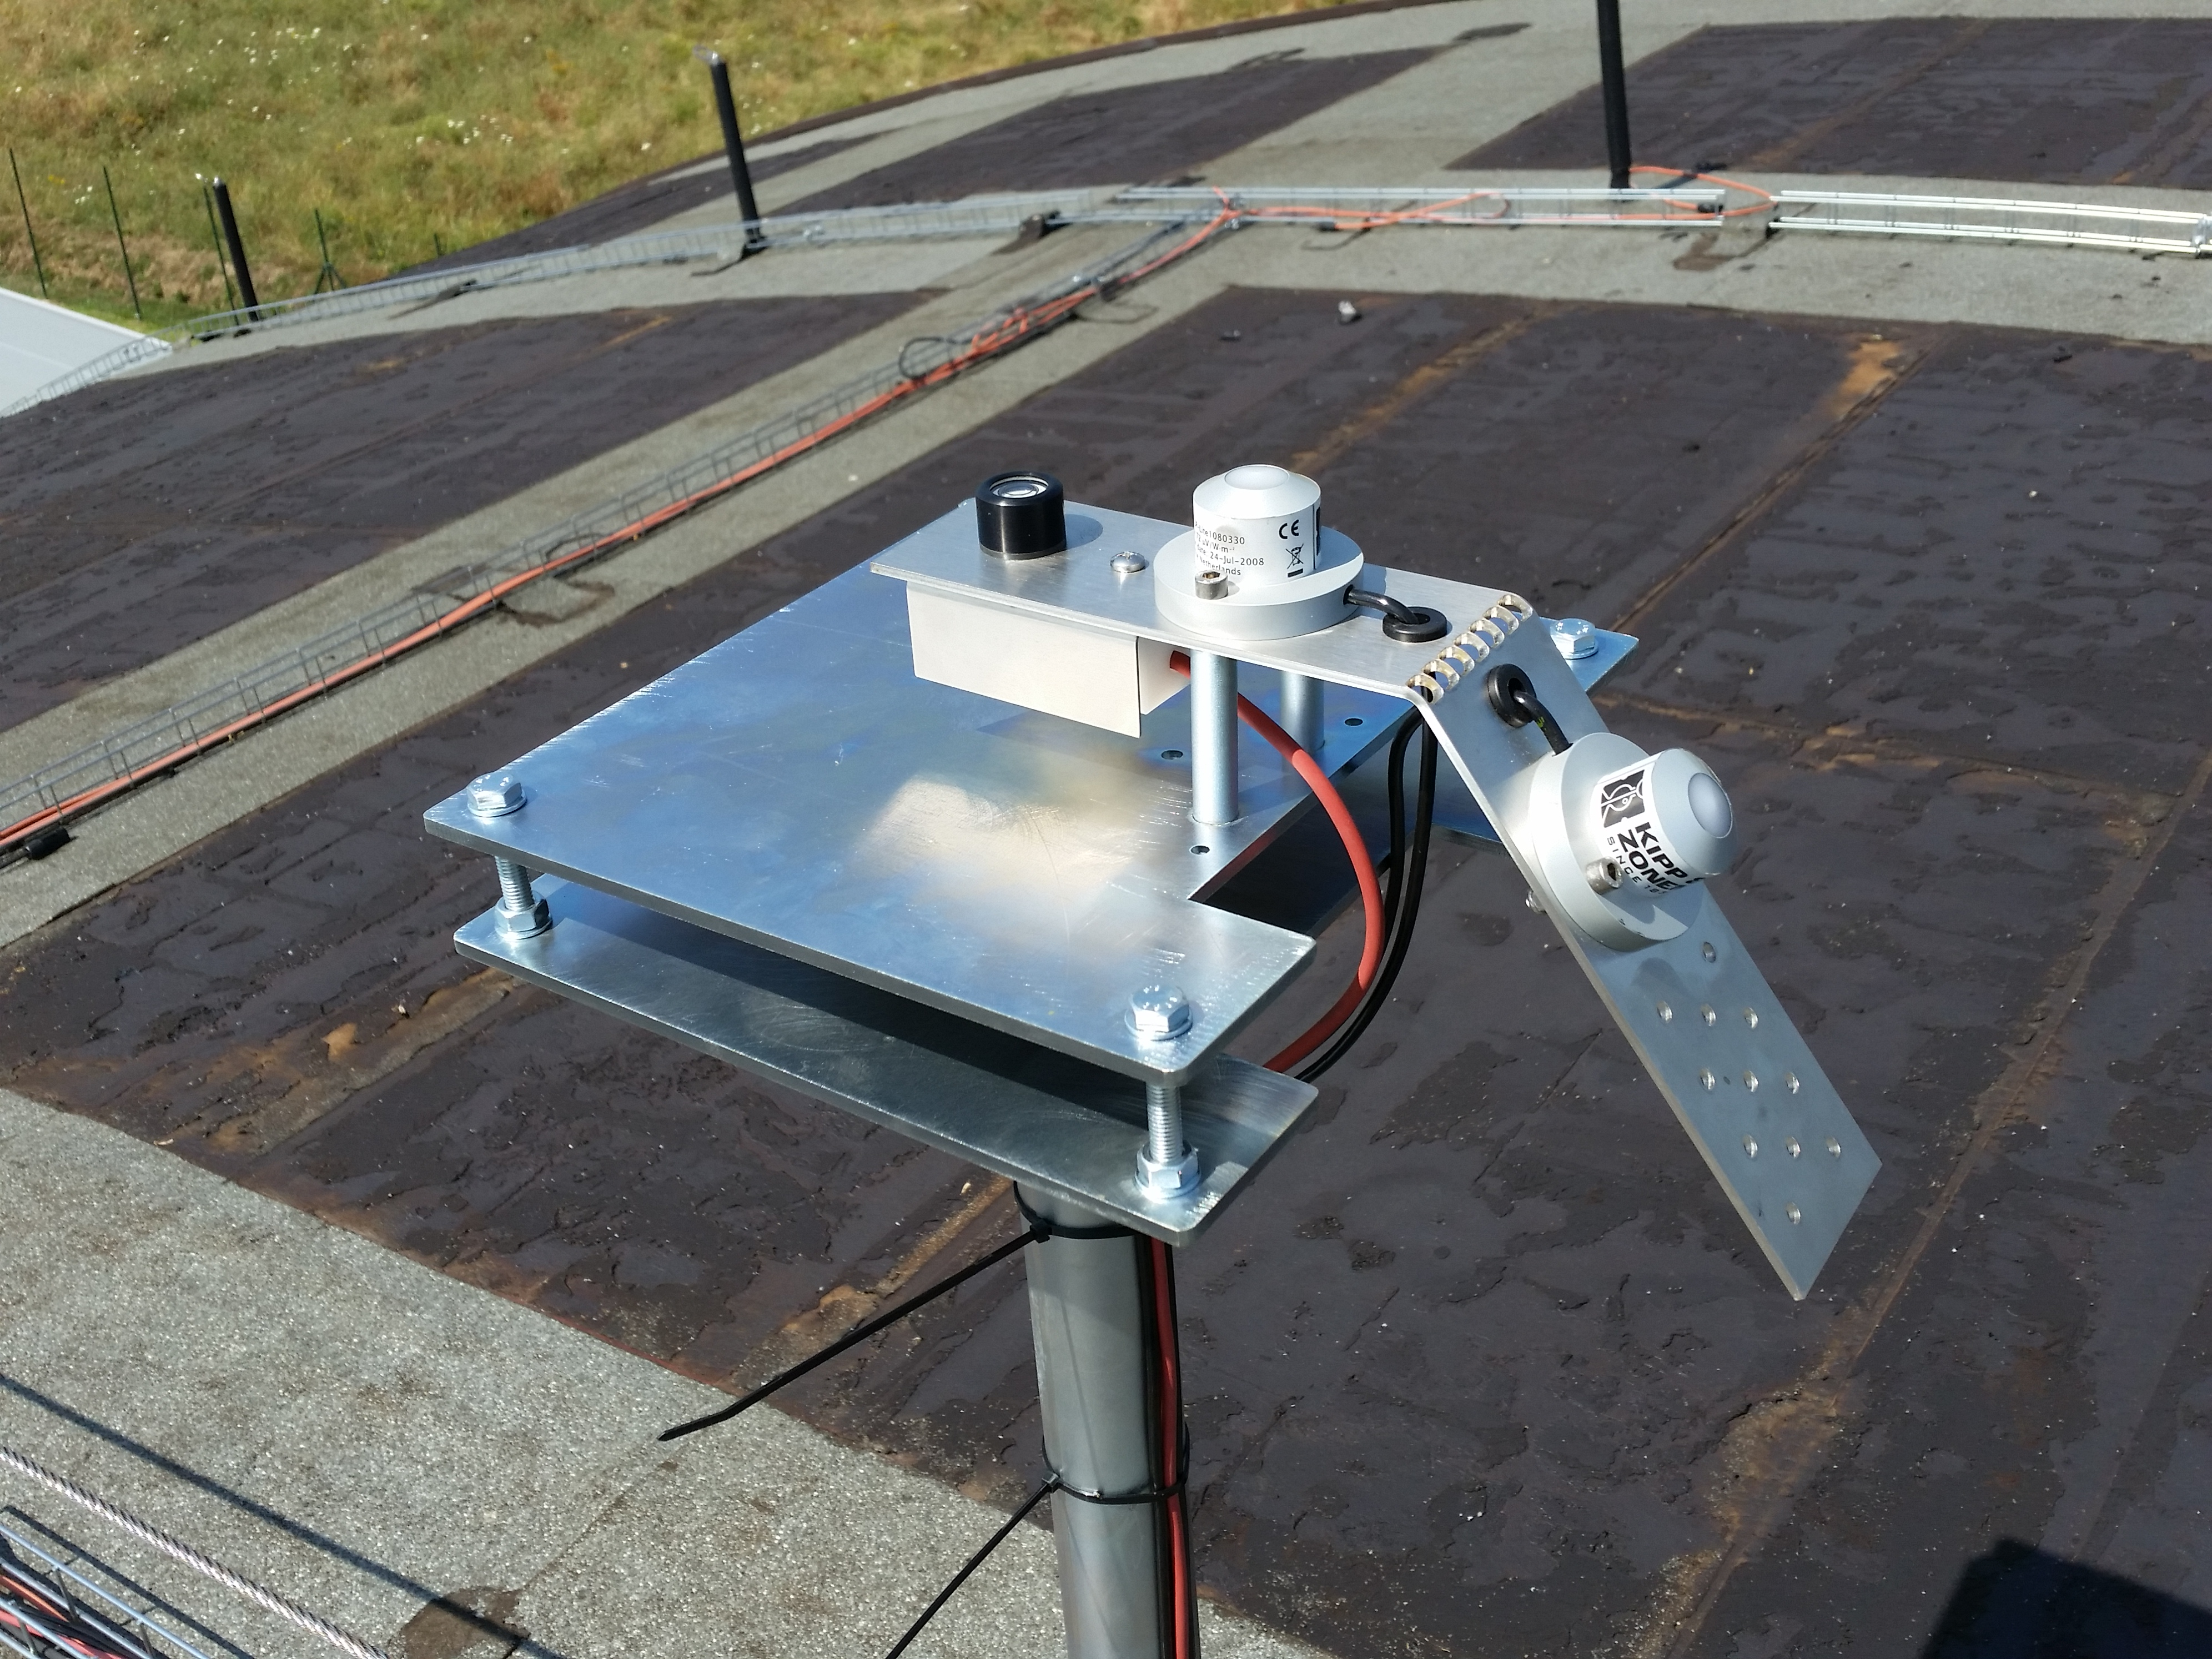
\includegraphics[scale=.3]{pyranometers}
\centering
\end{figure} 

\subsection{Acquired Data}
The camera system captures several images from the whole-sky every 8 seconds with different narrow exposure ranges. These images which are labeled according to capture time, are combined to create an HDR (High Dynamic Range) image for every sample time. The original narrow exposure images are generally deleted except the images at each hour time (i.e. around 7:00, 8:00, 9:00 etc.). Since capturing images at night is not useful for power prediction applications, camera is instructed to only take pictures during daytime (i.e. sunrise to sunset) which is obtained for that specific location for each day using mathematical models. Nevertheless, according to the captures images, this is not enough and still there are some black images taken at the minutes before sunrise and after sunset. Therefore, while processing the images on the application side, we exclude those images using a threshold on average pixel intensity of each image. This threshold is determined empirically. Using HDR images in the image processing step is one of the key differences between this study and related works specifically \cite{tSchmidt15}.

The pyranometers measure GHI values with the sample rate of 6 seconds. The temperature is also recorded with the  same sample rate. However, the generate power is measured and logged every 3 seconds. These different sample rate make it necessary to interpolate the available data to find the estimated data for a time which there is no data available. Therefore, we can assign total irradiance, temperature and generated power to any given image using its capture time. This data acquisition setup has been running since 7th July 2015 until present. However, there are some short periods of time (usually lasting several days up to two weeks) which one of the sensors (pyranometers or the camera) had problems or the power plant was not working to produce power data. Considering the relatively small sample rate (less than 8 seconds), the amount of recorded data is big enough to make those off-days negligible in data processing steps. The data used in this study spans from 15th July to 10 February, meaning that many summer, autumn and winter days are available in the dataset to make it a good representation for the whole year. 


\subsection{Sun positions and sun states in image}
Knowing position of sun is very important both in cloud segmentation and in irradiance estimation. First of all, since our images are from a wide-angle fisheye lens, they need to be transformed into geometric coordinates by an un-distortion algorithm to make them ready for further image processing steps including sun position, cloud segmentation and etc. This can be done by multiplying the raw image coordinates to camera transformation matrix which consists of intrinsic and extrinsic parameters of the camera system. As described in section \ref{sec:image_undistortion_schmidt}, intrinsic parameters are calculated using image of a chessboard\cite{fisheye_undistort} and extrinsic parameters are estimated using Kabsch algorithm\cite{Kabsch_alg} based on position of the sun appeared in the image versus the expected position of sun in image. The theoretical sun positions are calculated for the location of our PV plant site at every image time-stamp using NREL algorithm \cite{our_sun_position} in Matlab represented in unit sphere polar coordinates. As shown in Figure \ref{fig:sun_position_angles} this position is described as two angles (zenith and azimuth) which are converted to Cartesian coordinates using sphere to Cartesian conversion and later on are scaled to the image size to correspond with an image pixel. That pixel will be assumed as center of the sun.

\begin{figure}[h]
\caption{Sun position angles.  source:\cite{sun_angle_pic}}
\label{fig:sun_position_angles}
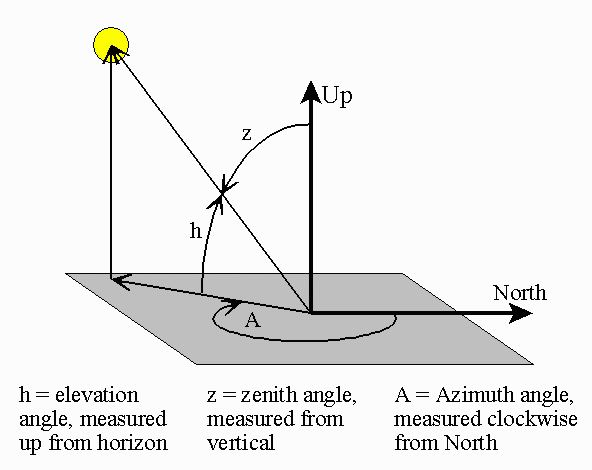
\includegraphics[scale=.5]{sun_angles}
\centering
\end{figure}

In cloud segmentation, which is not the focus of this study, sun position is used to treat pixels close to sun according to different threshold than other pixels. Furthermore, a sun state detection inspect the area around sun position to classify sun state in the image into following 4 categories:
\begin{itemize}
\item sun\_flag=4: indicating the sun is visible in the image and it appears as a star shape emitting 6 symmetric strong rays.
\item sun\_flag=3: indicating the sun is visible in the image and it appears as a star shape but with 5 or less symmetric strong rays.
\item  sun\_flag=2: indicating the sun is visible in the image but it does not appear as a star shape. Instead, it appears as a small black dot with no strong rays.
\item sun\_flag=1: indicating the sun is not visible in the image and it is either covered by clouds or the sun position is out of field of view in the image.
\item  sun\_flag=-1: indicating there is an unexpected situation around sun position, for example star shape sun is detected far away from expected sun position which could be because of strange cloud formations.
\end{itemize}
One sample for each one of these categories is depicted in Figure \ref{fig:sun_states}. We are able distinguish between this states thanks to HDR images, otherwise this fine classification would not be possible.

\begin{figure}[h]
\caption{Different sun states, from left to right: sun flag=4, 3, 2, 1 respectively.}
\label{fig:sun_states}
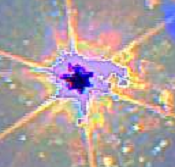
\includegraphics[scale=.5]{sun_flag_4}
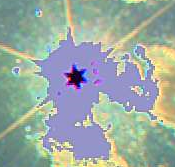
\includegraphics[scale=.5]{sun_flag_3}
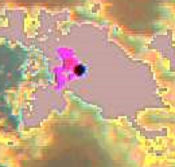
\includegraphics[scale=.5]{sun_flag_2}
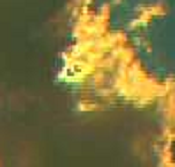
\includegraphics[scale=.5]{sun_flag_1}
\centering
\end{figure}

The variation of sun color in the images is so much that using Support Vector Machine for detecting sun is works very poorly. This issue is visible in Figure \ref{fig:sun_variation} which shows some clear sun samples from the images. Therefore, another approach using gray-scale images and geometrical symmetry detection is employed.

\begin{figure}[h]
\caption{Variation of sun appearance in the images.}
\label{fig:sun_variation}
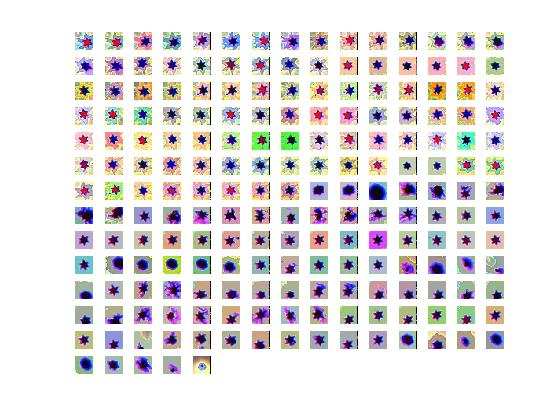
\includegraphics[scale=.7]{suns}
\centering
\end{figure}

Using these sun states along with the sun position in cloud segmentation algorithm, will lead to better segmentation results close to sun that is particularly a difficult area for cloud segmentation due to highly saturated pixels with different sky or cloud colors. In irradiance estimation which is the main focus of this study, sun position is used to create two specific feature vectors in a bounding circle around the sun. These features are explained section \ref{sec:img-features} in detail.

\subsection{Clear-sky irradiance model}
i.	Comparison of McClear \cite{mcclear_alg} model vs ineichen \cite{clear_sky_model} vs our measurements
ii.	clear-sky DNI is a good approximation for actual DNI. Showing some clear or cloudy days to prove this point.


\subsection{Estimating diffuse from pyranometers}
Using clearsun-flag and clear-sky DNI for calculating diffuse from tilted plate
We only consider images with complete visible sun or no sun at all.
ii.	Comparing tilted diffuse with diffuse from the main irradiance plate, then correcting tilted diffuse. Showing its robustness.
Show the result of relation of DNI DHI to irr1 irr2 with plots.

\subsection{Key image features affecting DHI}
\label{sec:img-features}
iii.	Investigate different parameters which affect diffuse
\subsubsection{Discuss cloud coverage geometrical polar feature around sun and also the whole image}
\subsubsection{Discuss saturation detection algorithm and its results}


iv.	Show their correlation to diffuse, discuss cases based on images and corresponding irradiance components


\subsection{Learning the relation between image features and DHI}
Regression, or svorim method for estimation
Compare to other method to regress, or penalty [no result]



\subsection{Translating irradiance to power}
\subsubsection{Estimating shadow ratio on the plant site}
Projecting plant coordinates into the sky using assumed cloud height
Adaptation to smooth changes of power by using the histogram of irradiance over past 30 minutes

